%% Beispiel-Präsentation
\documentclass[navbaroff,4:3]{kitbeamer} 

\usepackage{tikz}
\usepackage{tikz-layers}
\usetikzlibrary{automata,fit,shapes,positioning,patterns}
\usepackage{fontawesome5}

\newcommand{\kit}[1]{\textcolor{kit-green100}{#1}}
\newcommand{\kitbf}[1]{\kit{\bf #1}}

%% Titelbild
\titleimage{key-wide}

%% Gruppenlogo
\grouplogo{} 

%% Gruppenname
\groupname{Institute of Theoretical Informatics}

% Beginn der Präsentation

\title{Specifying Components with Automata}
\subtitle{for the VerifyThis Long Term Challenge} 
\author{Mattias Ulbrich and Alexander Weigl}

\date[]{\today}

\begin{document}

%Titelseite
%KITtitleframe

\begin{frame}{Goal}

  \large

  \kitbf{It's about:} Show how an automaton specification can be used for Java
  component specification.

  \vfill

  \kitbf{It's \emph{not} about} inventing another automaton language.
  
\end{frame}

\begin{frame}[fragile]{Hagrid as a component}

  % \begin{tikzpicture}[
  %   database/.style={
  %     cylinder,
  %     cylinder uses custom fill,
  %     cylinder body fill=white,
  %     cylinder end fill=white,
  %     shape border rotate=90,
  %     aspect=0.25,
  %     draw
  %   }, thick]
    
  %   \node (U) {\Huge\faUser};
  %   \node[below=.2 of U] (UD) {User};
    
  %   \node[right=2 of U,draw,rectangle,minimum width=4em,minimum height=6em] (WS) {\Huge \faServer};
  %   \node[above=.2 of WS] (WSD) {Frontend};
    
    
  %   \node[right=1.5 of WS,draw,rectangle,
  %   text centered, text depth=.25ex, %fill=yellow!50,
  %   pattern=crosshatch dots gray,
  %   minimum width=5em,minimum height=6em] (B)
  %   {\Huge\faCogs};
  %   \node[above=.2 of B] (BD) {Backend};
    
    
  %   \node[right=of B,draw,database,
  %   text centered,text depth=1ex,
  %   text width=4em,text height=2em] (DB) {\Huge\faKey};
  %   \node[above=.2 of DB] (DBD) {Database};
    
  %   \newcommand\request[2]{%
  %     \draw[->]
  %     ([yshift=#1]U.east)
  %     -- node[above,pos=.9,anchor=south east]{\small\texttt{#2}}
  %     ([yshift=#1]WS.west)
  %     ([yshift=#1]WS.east)
  %     --
  %     ([yshift=#1]B.west);
  %   }
    
  %   \foreach \x/\y in {22.5/get,7.5/add,-7.5/del,-22.5/confirm}{%
  %     \request{\x}{\y}
  %   }
    
    
  %   \draw[->]
  %   (B.south) -- ([yshift=-15]B.south) -| node[below,pos=.1]{\texttt{confirm?}} ([yshift=-20]U.south);
    
  %   \draw[<->] (B) -- (DB);
  % \end{tikzpicture}

  \begin{center}
    \begin{tikzpicture}[
      database/.style={
        cylinder,
        cylinder uses custom fill,
        cylinder body fill=white,
        cylinder end fill=white,
        shape border rotate=90,
        aspect=0.25,
        draw
      }, thick]
      
      \node (U) {\Huge\faUser};
      \node[below=.2 of U] (UD) {User};
      
      \node[right=2 of U,draw,rectangle,minimum width=4em,minimum height=6em]
      (WS) {
        \scalebox{.5}{%
        \begin{tikzpicture}[->,auto,y=1.5cm]
          \begin{scope}[local bounding box=a]
            \node[align=left] at (-1.8, 3.8) {\emph{Globals:} $\mathit{Ks} : \mathit{set}(\mathtt{String})$};
            
            \begin{scope}[local bounding box=b]
              \node[align=left, text width=2cm] at (-1.8, 2.5)
               {\emph{Locals:} \\
                 $K: \mathtt{String}$ \\
                 $V: \mathtt{String}$ \\
                 $C: \mathtt{String}?$};
              
               \node[state,fill=black, circle,text height=1em,text width=1ex] (empty)  at (1, 3) {} ;
              \node[state] (registered) at (1, 2) {R};
              \node[state] (confirmed) at (1, 1) {C};
              \node[state, accepting] (finished) at (0,0) {F};
              
              \path
              (empty)      edge node[align=left, text width=6cm]
              {\texttt{register}(k,v)=c,  k$\not\in$Ks /\\
                V:=v; C:=c; K:=k; Ks:=Ks$\cup$\{k\}} (registered)
              (registered) edge node {\texttt{confirm}(c), c=C} (confirmed)
              (registered) edge[swap, bend right] node {\texttt{delete}(k), k=K} (finished)
              (confirmed)  edge node {\texttt{delete}(k), k=K} (finished)
              (confirmed)  edge[loop right] node {\texttt{get}(k)=v, k=K / ==> v=V} (confirmed);
            \end{scope}
          \end{scope}
          \node [fit=(a),inner sep=2pt,draw,rounded corners] {};
          \node [fit=(b),inner sep=2pt,draw,rounded corners] {};
        \end{tikzpicture}
        }
      };

      \newcommand\request[2]{%
        \draw[->]
        ([yshift=#1]U.east)
        -- node[above,pos=.9,anchor=south east]{\small\texttt{#2}}
        ([yshift=#1]WS.west);
      }
      
      \foreach \x/\y in {22.5/get,7.5/add,-7.5/del,-22.5/confirm}{%
        \request{\x}{\y}
      } 
      
      
      % \draw[->]
      % (B.south) -- ([yshift=-15]B.south) -| node[below,pos=.1]{\texttt{confirm?}} ([yshift=-20]U.south);
      
      %draw[<->] (B) -- (DB);
    \end{tikzpicture}
  \end{center}

  \begin{itemize}
  \item operations receive and return immutable data
  \item operations modify a self-contained state 
  \item not every operation may be invoked at all times
  \end{itemize}
\end{frame}

% Inhaltsverzeichnis
\begin{frame}{Specifying Hagrid with an Automaton}

  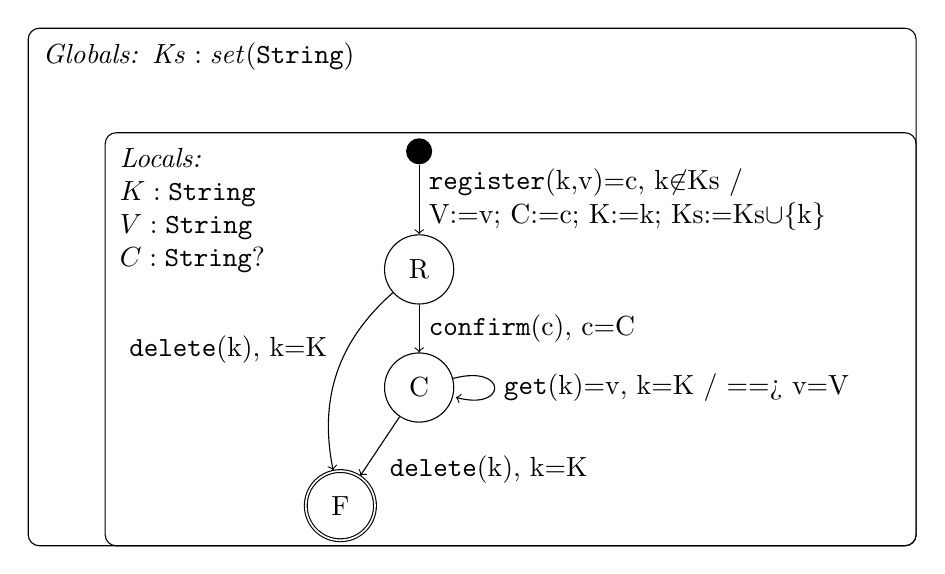
\begin{tikzpicture}[auto, ->, y=1.5cm]
    \begin{scope}[local bounding box=a]
      \node[align=left] at (-1.8, 3.8) {\emph{Globals:} $\mathit{Ks} : \mathit{set}(\mathtt{String})$};
      
      \begin{scope}[local bounding box=b]
        \node[align=left, text width=2cm] at (-1.8, 2.5)
        {\emph{Locals:} \\
          $K: \mathtt{String}$ \\
          $V: \mathtt{String}$ \\
          $C: \mathtt{String}?$};
        
        \node[fill=black, circle] (empty) at (1, 3) {};
        \node[state] (registered) at (1, 2) {R};
        \node[state] (confirmed) at (1, 1) {C};
        \node[state, accepting] (finished) at (0,0) {F};
        
        \path
        (empty)      edge node[align=left, text width=6cm]
        {\texttt{register}(k,v)=c,  k$\not\in$Ks /\\
          V:=v; C:=c; K:=k; Ks:=Ks$\cup$\{k\}} (registered)
        (registered) edge node {\texttt{confirm}(c), c=C} (confirmed)
        (registered) edge[swap, bend right] node {\texttt{delete}(k), k=K} (finished)
        (confirmed)  edge node {\texttt{delete}(k), k=K} (finished)
        (confirmed)  edge[loop right] node {\texttt{get}(k)=v, k=K / ==> v=V} (confirmed);
      \end{scope}
    \end{scope}
    \node [fit=(a),inner sep=2pt,draw,rounded corners] {};
    \node [fit=(b),inner sep=2pt,draw,rounded corners] {};
  \end{tikzpicture}
\end{frame}


\newcommand\autom[6]{
  \node[align=left, text width=2cm] at (-0., 2.9)
  {\emph{Locals:} \\
    $K = \kit{#1}$ \\
    $V = \kit{#2}$ \\
    $C = \kit{#3}$};
  
  \node[fill=black, circle] (empty) at (1, 3) {};
  \node[state,#4] (registered) at (1, 2) {R};
  \node[state,#5] (confirmed) at (1, 1) {C};
  \node[state,accepting,#6] (finished) at (0,0) {F};
  
  \path
  (empty)      edge (registered)
  (registered) edge (confirmed)
  (registered) edge[bend right]  (finished)
  (confirmed)  edge (finished)
  (confirmed)  edge[loop right] (confirmed); 
}

\begin{frame}{Example state}
  \begin{tikzpicture}[auto, ->, y=1.5cm]
    \begin{scope}[local bounding box=o]
      \node[align=left] at (0, 4) {\emph{Globals:} $\mathit{Ks} = \kit{\{ a@x, b@x, c@x \}}$};
      
      \begin{scope}[xshift=-1cm,local bounding box=a]    
        \autom{a@x}{KEY1}{CONF1}{}{fill=kit-green50}{}
      \end{scope}
      
      \begin{scope}[xshift=3cm,local bounding box=b]
        \autom{b@x}{KEY2}{CONF2}{}{fill=kit-green50}{}
      \end{scope}
      \begin{scope}[xshift=7cm,local bounding box=c]
      \autom{c@x}{KEY3}{CONF3}{fill=kit-green50}{}{}
      \end{scope}
    \end{scope}

    \node [fit=(a),inner sep=2pt,draw,rounded corners] {};
    \node [fit=(b),inner sep=2pt,draw,rounded corners] {};
    \node [fit=(c),inner sep=2pt,draw,rounded corners] {};
    \node [fit=(o),inner sep=2pt,draw,rounded corners] {};
    \end{tikzpicture}
  
\end{frame}

\begin{frame}{Semantics}

  The automaton is a \textbf{stateful contract} for the component.

  \vfill
  
  It specifies
  \begin{itemize}
  \item which operations 
  \item with which parameters are allowed,
  \item and which operations are not allowed
  \end{itemize}
  depending on the current state.

  \begin{block}{Trace semantics}
    The semantics of a specification is the set of all traces of the
    automaton that satisfy all conditions.

    Trace: Sequence of parametrised operation invocations
  \end{block}
\end{frame}



% XXX weigl: Folie überladen, was ist die Botschaft?
\begin{frame}{The two faces of the interface}
  \begin{tikzpicture}
    \begin{scope}[local bounding box=o]
    \node[anchor=west] at (-5.6, 2.5) {\textbf{Outside:} Environment};
    \node[anchor=west] at (0, 2) {\textbf{Inside:} the component};

    \node[anchor=north west, text width=4cm] at (-5.6, 1.5) { \small
      \textbf{Obligations:}
      \begin{itemize}
      \item temporal properties
      \item protocol adherence (multi-component)
      \end{itemize}

      \textbf{Gains:}
      \begin{itemize}
      \item sound abstract from code
      \end{itemize}

        \textbf{Construct:}\\automata/proc algebra};
      
      \begin{scope}[local bounding box=i]
        \node[anchor=west] at (0, 2) {\textbf{Inside:} the component};

    \node[anchor=north west, text width=3cm] at (2, 1.5) { \small
      \textbf{Obligations:}
      \begin{itemize}
      \item contract conformance
      \end{itemize}

      \textbf{Gains:}
      \begin{itemize}
      \item temporal/protocol properties
      \end{itemize}

      \textbf{Construct:} contracts and ghost code};
      \end{scope}
    \end{scope}

    \begin{scope}[on background layer]
      \node[fit=(o),draw,fill=kit-blue15,rounded corners]{};
      \node[fit=(i),draw,fill=kit-green15,rounded corners]{};
    \end{scope}
    
    %\draw[thick, rounded corners, fill=green!15] (-5.6,3) rectangle (5.6,-3);
    %\draw[thick, rounded corners, fill=blue!15] (0,2.5) rectangle (5.1,-2.5);

  
   \node at (0,0) {\includegraphics[width=4cm]{automaton.png}};
  \end{tikzpicture}
\end{frame}

\begin{frame}{Demo?}
  
\end{frame}

\begin{frame}{Verification}
Deductive Verification, Modularity?
\end{frame}

\end{document}
